\documentclass[12pt]{article}

\usepackage{graphicx}
%\usepackage{float}
%\usepackage{subfig}
%\usepackage{array}
\usepackage{amsmath}
\usepackage{amsfonts}
\usepackage{amsthm}



\newcommand{\bm}[1]{\boldsymbol{#1}}

\newcommand{\ones}{\mathbf 1}
\newcommand{\zeros}{\mathbf 0}
\newcommand{\reals}{{\mbox{\bf R}}}
\newcommand{\integers}{{\mbox{\bf Z}}}
\newcommand{\symm}{{\mbox{\bf S}}}  % symmetric matrices

\newcommand{\nullspace}{{\mathcal N}}
\newcommand{\range}{{\mathcal R}}
\newcommand{\Rank}{\mathop{\bf Rank}}
\newcommand{\Tr}{\mathop{\bf tr}}
\newcommand{\diag}{\mathop{\bf diag}}
\newcommand{\lambdamax}{{\lambda_{\rm max}}}
\newcommand{\lambdamin}{\lambda_{\rm min}}

\newcommand{\Expect}{\mathop{\bf E{}}}
\newcommand{\Prob}{\mathop{\bf Prob}}




\title{Maximum Load Determination of a Truss by Linear Programming}
\author{Shalom D. Ruben}
\date{}

\begin{document}
\maketitle

\begin{abstract}
In this report we describe how the maximum load of a predefined truss can be calculated by linear programming (LP).  An example steel truss is given and the solution to two different load states are presented with numerical results.
\end{abstract}

\section{Introduction}
Numerical optimization is a tool for solving complex problems that would otherwise be extremely difficult to solve by other means.  We present a structural application and formulate it as an LP so that it can be solved efficiently with the state-of-the-art solvers that are available including linprog() in Matlab.\\

Take for example the truss shown in Figure \ref{fig:Example} (found in \cite{EngOpt}), which shows a load being equally supported by the truss at two nodes (joints).  In a situation as this, an engineer may be interested in the maximum load ($P_\textrm{max}$) that this truss can support in order to define a ``safe" load which is a factor of the maximum load defined by the following equation:
\begin{equation}
P_\textrm{max} = N*P_\textrm{safe}
\end{equation}
where $N$ is known as the ``factor-of-safety".  Values for factor-of-safety depend on many factors but some example are $1.4$ for commercial aircrafts and $11$ for public elevators \cite{MachineDesign}.\\

In the following sections we will describe the LP formulation for finding the maximum load for a given truss.  We will also solve this problem, numerically, for two different load cases.

\begin{figure}[htb!]
	\begin{center}
		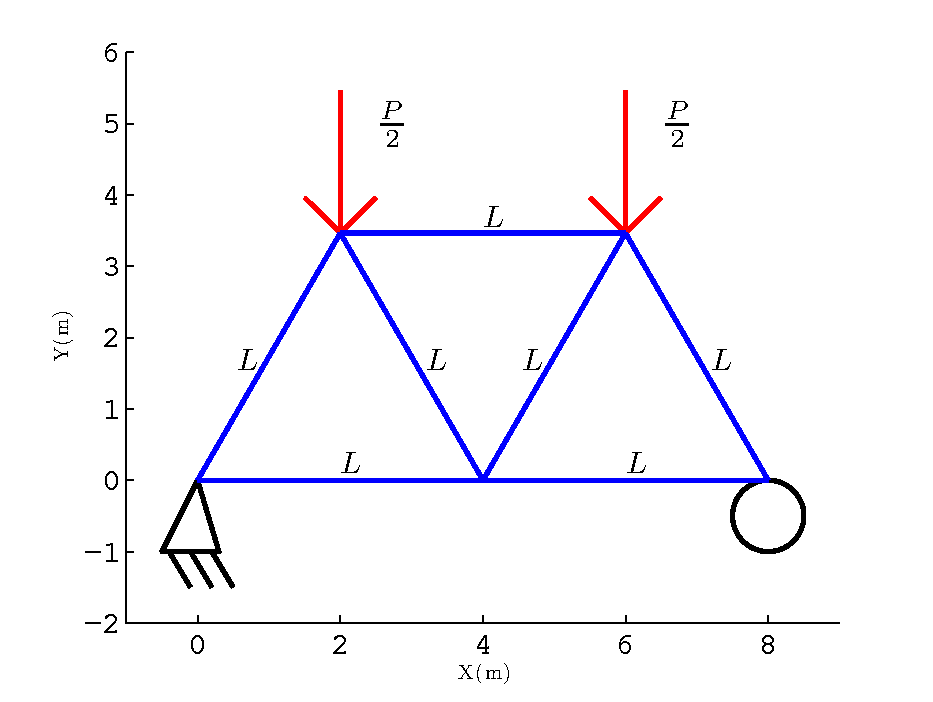
\includegraphics[width=1\textwidth]{TrussFS}
	\end{center}
	\caption{Example Truss}
	\label{fig:Example}
\end{figure}

\section{LP formulation}
To formulate the LP we need to describe in some detail the cost function and constraints.  We are trying to find the maximum $P$ that satisfies the constraints, so maximizing $P$ or minimizing $-P$ is our cost function.  We have a few constraints, the simplest of which is that the absolute value of the stress at each member ($\sigma_i$, for i=$1\cdots m$ bars) cannot be greater than the yield Strength ($S_y$) of the material:
\begin{equation}
|\sigma_i| \leq S_y
\end{equation}
where stress is the force ($u_i$) over the cross-sectional area ($A$, assumed to be constant):
\begin{equation}
\sigma_i = \frac{u_i}{A}
\end{equation}
These equations can be reorganized to give our final constraint that governs the failure of each member:
\begin{equation}
 -A*S_y \leq u_i \leq A*S_y
\end{equation}
or
\begin{equation}
\left[
\begin{array}{rr}
\bm{I} & \bm{0}\\
-\bm{I} & \bm{0}
\end{array}
\right]
x \leq
\left[
\begin{array}{c}
A*S_y\\
A*S_y
\end{array}
\right]
\end{equation}
where
\begin{equation}
x = \left[
\begin{array}{c}
u_1\\
u_2\\
\vdots\\
u_m\\
P
\end{array}
\right]
\end{equation}

Finally, we need to deal with the force equilibrium constraints where the sum of the forces at a free joint, in $x$ and $y$, are equal to zero.  The references for building these equality constraints are found in \cite{236A} and the author's lecture on ``Structural Optimization".  These give us equality constraints that need to be determined using the technique found in the references:
\begin{equation}
\hat{A}x=\hat{b}
\end{equation}
Our LP formulation is now fully defined as:
\begin{eqnarray}
\begin{array}{ll}
\mbox{minimize} &\quad \hat{c}^Tx\\
\mbox{subject to} & \quad \hat{A}x=\hat{b}\\
&\left[
\begin{array}{cc}
\phantom{-}\bm{I} & \bm{0}\\
-\bm{I} & \bm{0}
\end{array}
\right]
x \leq
\left[
\begin{array}{c}
A*S_y\\
A*S_y
\end{array}
\right]
\end{array}
\label{eqn:LP}
\end{eqnarray}
where
\begin{equation}
\hat{c} =
\left[
\begin{array}{r}
\bm{0}\\
-1
\end{array}
\right]
\end{equation}

It is possible to turn the equality constraints $\hat{A}x=\hat{b}$ into two inequality constraints and merge them with the other inequality constraints, but since the linprog() function in Matlab allows equality constraints along with inequaility constraints as an input, they will be left alone.

\section{Numerical Results}
Now that the LP formulation is finished, we will look at a specific truss geometry with two different load cases.  For both of these cases, the constants defining the truss can be found in Table \ref{tab:Constants}.
\begin{table}[htb!]
\caption{Constants For Truss Problems}
\label{tab:Constants}
\begin{center}
  \begin{tabular}{@{} |c|c|c| @{}}
    \hline
     Constant\ & Symbol\ & Value\\
    \hline
\hline
   Yield Strength\ & $S_y$&1.85MPa \\
\hline
  Area\ &$A$&5.475$\times10^{-4}$ m$^2$ \\
    \hline
  Length\ &$L$&4 m\\
    \hline
  \end{tabular}
\end{center}
\end{table}
Also the numbering system of $N=5$ nodes and $m=7$ truss members can be found in Figure \ref{fig:NodesBars}.
\begin{figure}[htb!]
	\begin{center}
		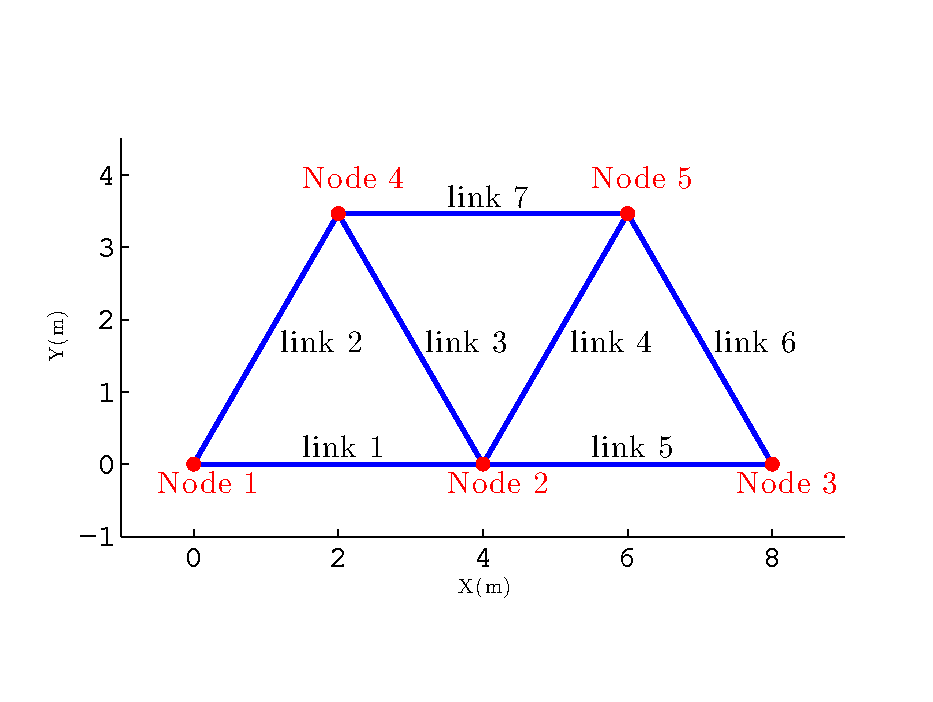
\includegraphics[width=1\textwidth]{TrussFSNodesBars2}
	\end{center}
	\caption{Numbering system for the Bars and Nodes of the example truss}
	\label{fig:NodesBars}
\end{figure}
Notice also that since the truss is made of equilateral triangles, and that many of the bars make 30-60-90 triangles, we will find a lot of force components to be $\pm \sqrt{3}u_i/2$ and $\pm u_i/2$.  To reduce clutter of the coming matrices the following constants are defined:
\begin{eqnarray}
c_{60} &=& \frac{\sqrt{3}}{2}\\
c_{30} &=& \frac{1}{2}
\end{eqnarray}

\subsection{Load State 1}
The first load we will analyze is shown in Figure \ref{fig:Load1} which is a repeat of the example truss already shown in Figure \ref{fig:Example}.
\begin{figure}[htb!]
	\begin{center}
		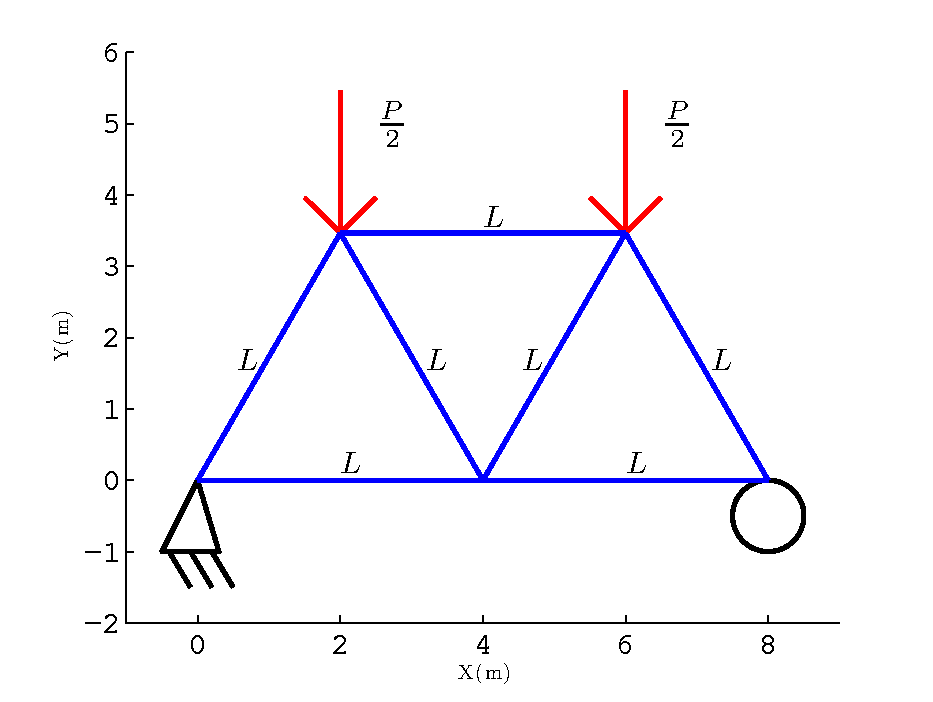
\includegraphics[width=1\textwidth]{TrussFS}
	\end{center}
	\caption{Load State 1}
	\label{fig:Load1}
\end{figure}
As described earlier, a load $P$ is equally distributed in the $y$ direction between nodes 4 and 5.  The only constraints that need to be defined are the force equilibrium constraints for the free nodes.  It is obvious that there are at least 3 free nodes giving 6 constraints, but the rolling support is something to pay attention to.  The rolling support is fixed only in the $y$ direction, so the $x$ direction is a single free node, rather than 2, and will bring the total number of equality constraint equations to 7.  For this example, and by methods in references, it can be shown that the equality constraints are:
\begin{equation}
\left[
\begin{array}{cccccccc}
-1  & 0             & -c_{30}  &  c_{30}   &1     &0            &0   &0\\
0   & 0             &c_{60}     &c_{60}     &0     &0            &0   &0\\
0   &0              &0              &0              &-1    &-c_{30}  &0   &0\\
0   &-c_{30}   &c_{30}     &0              &0     &0             &1   &0\\
0   &-c_{60}   &-c_{60}    &0              &0    &0              &0   &-c_{30} \\
0   & 0             &0              &-c_{30}    &0    &c_{30}    &-1  &0\\
0   &0              &0              &-c_{60}    &0    &-c_{60}   &0   &-c_{30}
\end{array}
\right]
\left[
\begin{array}{c}
u_1\\
u_2\\
u_3\\
u_4\\
u_5\\
u_6\\
u_7\\
P
\end{array}
\right]
=
\left[
\begin{array}{c}
0\\
0\\
0\\
0\\
0\\
0\\
0\\
0
\end{array}
\right]
\end{equation}
After solving the LP (see code found in appendix), the solution vector $x^\star$ is given as:
\begin{equation}
\nonumber
x^\star = 10^4
\left[
\begin{array}{r}
0.5064\\
-1.0129\\
0\\
0\\
0.5064\\
-1.0129\\
-0.5064\\
1.7544
\end{array}
\right]
\end{equation}
$P_\textrm{max}$ is given as $x^\star(8)=17544$ Newtons (N) or almost 4000 pounds (lbs).  Also, it is interesting to notice that truss members 3 and 4 are not needed, which would give you the truss geometry found in Figure \ref{fig:Result}.
\begin{figure}[htb!]
	\begin{center}
		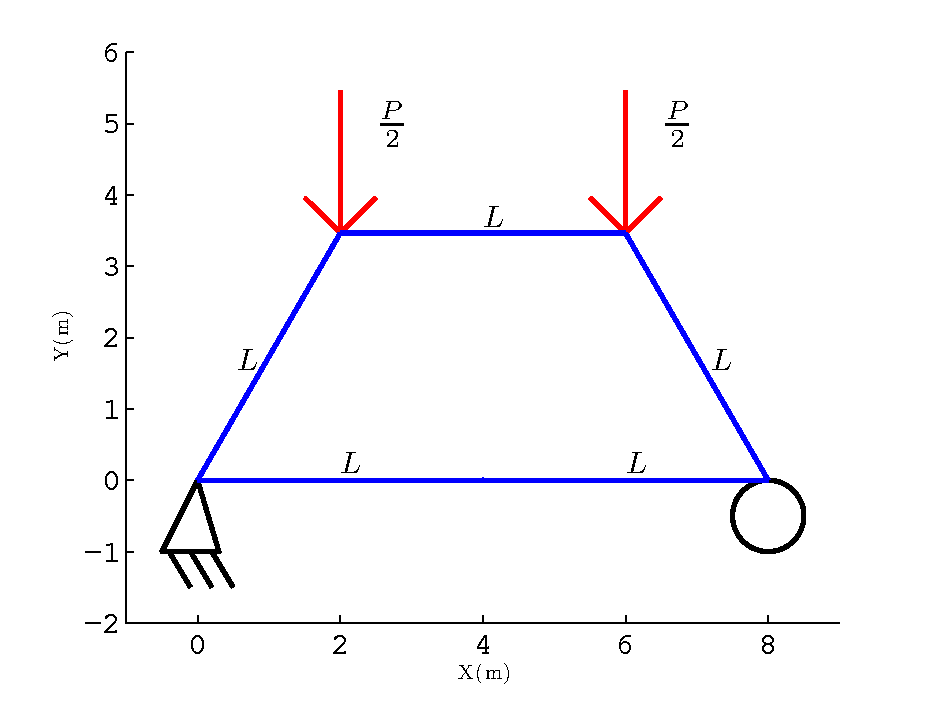
\includegraphics[width=1\textwidth]{TrussFS3}
	\end{center}
	\caption{The results of the LP, for load case 1, shows that links 3 and 4 are not necessary}
	\label{fig:Result}
\end{figure}

\newpage
\subsection{Load State 2}
This second load case is shown in Figure \ref{fig:Load2}.
\begin{figure}[htb!]
	\begin{center}
		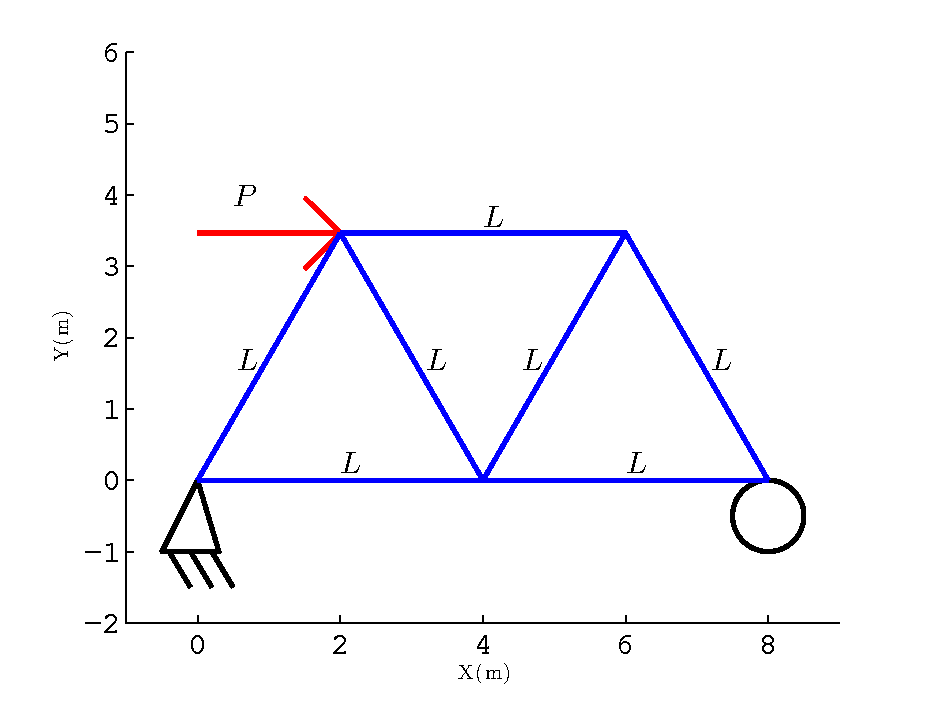
\includegraphics[width=1\textwidth]{TrussFS2}
	\end{center}
	\caption{Load State 2}
	\label{fig:Load2}
\end{figure}
In this case, the force is purely in the $x$ direction located at node 4.  The force equilibrium equality constraints for this problem are:
\begin{equation}
\left[
\begin{array}{cccccccc}
-1  & 0             & -c_{30}  &  c_{30}   &1     &0            &0   &0\\
0   & 0             &c_{60}     &c_{60}     &0     &0            &0   &0\\
0   &0              &0              &0              &-1    &-c_{30}  &0   &0\\
0   &-c_{30}   &c_{30}     &0              &0     &0             &1   &1\\
0   &-c_{60}   &-c_{60}    &0              &0    &0              &0   &0\\
0   & 0             &0              &-c_{30}    &0    &c_{30}    &-1  &0\\
0   &0              &0              &-c_{60}    &0    &-c_{60}   &0   &0
\end{array}
\right]
\left[
\begin{array}{c}
u_1\\
u_2\\
u_3\\
u_4\\
u_5\\
u_6\\
u_7\\
P
\end{array}
\right]
=
\left[
\begin{array}{c}
0\\
0\\
0\\
0\\
0\\
0\\
0\\
0
\end{array}
\right]
\end{equation}
After solving the LP, the solution vector $x^\star$ is given as:
\begin{equation}
\nonumber
x^\star = 10^4
\left[
\begin{array}{r}
    1.0129\\
    0.6752\\
   -0.6752\\
    0.6752\\
    0.3376\\
   -0.6752\\
   -0.6752\\
    1.3505
\end{array}
\right]
\end{equation}
As you can see from the results of this problem, every link is crucial to an external force in the $x$ direction versus in the $y$ direction as shown in the previous case.

\section{Conclusion}
In conclusion, we presented the LP formulation for finding the maximum load for a given truss geometry and force state.  It was shown through two numerical example how to use the LP formulation to get the maximum load.  It was interesting that under a specific load case, some members support no load an therefore were not needed.  Further constraints in the future could be added, such as deflection constraints at a specific node, or replacing the roller support with a pin support and analyzing how the members distribute the loads.

\appendix
\section{Code}
\subsection{Solving LP}
\begin{verbatim}
%%%%%%%%% LINEAR PROGRAM %%%%%%%%%%%%%%%%

%%% Maximize P
c_hat = [zeros(Links,1);1];

%%% Subject to the Equilibrium constraints
%%% Aeq * x = beq
%%%
Aeq    = [-1   0 -c1  c1   1   0  0   0;
           0   0  c2  c2   0   0  0   0;
           0   0   0   0  -1 -c1  0   0;
           0 -c1  c1   0   0   0  1   0;
           0 -c2 -c2   0   0   0  0 -c1;
           0   0   0 -c1   0  c1 -1   0;
           0   0   0 -c2   0 -c2  0 -c1];

beq = zeros(7,1);

%%% Subject to the Failure constraints
%%% A_hat2 * x <= b_hat2 (or -A*Sy<=u_i<=A*Sy)
%%%
A_hat = [eye(Links) zeros(Links,1);
         -eye(Links) zeros(Links,1)];

b_hat = [A*Sy*ones(Links,1);
          A*Sy*ones(Links,1)];

[x_star J_star Flag]=linprog(-c_hat,A_hat,b_hat,Aeq,beq);
\end{verbatim}

\subsection{Plotting}
\begin{verbatim}
%%%%%%%%%%% FIGURE 4 %%%%%%%%%%%%%%%%%%%%%%
%%
figure,
hold on

%%% Plot Links
plot([x(1) x(2)],[y(1) y(2)],'Linewidth',2)
plot([x(1) x(4)],[y(1) y(4)],'Linewidth',2)
plot([x(2) x(3)],[y(2) y(3)],'Linewidth',2)
plot([x(2) x(4)],[y(2) y(4)],'Linewidth',2)
plot([x(2) x(5)],[y(2) y(5)],'Linewidth',2)
plot([x(3) x(5)],[y(3) y(5)],'Linewidth',2)
plot([x(4) x(5)],[y(4) y(5)],'Linewidth',2)

%%% Draw Nodes
plot(x,y,'r.','MarkerSize',20)

%%% Figure Additions
text(3.5,3.7,'link 7','interpreter','Latex','FontSize',15)
text(1.2,1.7,'link 2','interpreter','Latex','FontSize',15)
text(7.2,1.7,'link 6','interpreter','Latex','FontSize',15)
text(3.2,1.7,'link 3','interpreter','Latex','FontSize',15)
text(5.2,1.7,'link 4','interpreter','Latex','FontSize',15)
text(1.5,.25,'link 1','interpreter','Latex','FontSize',15)
text(5.5,.25,'link 5','interpreter','Latex','FontSize',15)

text(-.5,-.25,'Node 1','interpreter','Latex','FontSize',15,'Color','r')
text(3.5,-.25,'Node 2','interpreter','Latex','FontSize',15,'Color','r')
text(7.5,-.25,'Node 3','interpreter','Latex','FontSize',15,'Color','r')
text(1.5,4*c2+.5,'Node 4','interpreter','Latex','FontSize',15,'Color','r')
text(5.5,4*c2+.5,'Node 5','interpreter','Latex','FontSize',15,'Color','r')

xlabel ('X(m)','interpreter','Latex')
ylabel ('Y(m)','interpreter','Latex')

set(gca,'FontSize',15)
set(gca,'FontName','cmr12')

axis equal
axis([-1 9 -1 4.5])

%%%%%%% END FIGURE 4 %%%%%%%%%%%%%%%%%%%%%%%%%%%%
\end{verbatim}

\bibliographystyle{plain}
\bibliography{SampleReport}

\end{document}
